\chapter{Introducción Específica} % Main chapter title

\label{Chapter2}

En este capítulo se identifican aspectos relevante de la planificación . Asimismo, se describen las herramientas empleadas para la realización de este trabajo.

%----------------------------------------------------------------------------------------
%	SECTION 1
%----------------------------------------------------------------------------------------
\section{Requerimientos}
\label{sec:requerimientos}

A continuación se enumeran los requerimientos del proyecto:

\begin{enumerate}
  \item Requerimientos de documentación:
   \begin{enumerate}
     \item Se debe generar un Memoria Técnica con la documentación de ingeniería detallada.
	   \item Se debe generar un documento de casos de prueba.
	 \end{enumerate}
	\item Requerimientos funcionales del sistema:
	\begin{enumerate}
		\item El sistema debe adquirir datos de un array de sensores de temperatura a intervalos regulares con un período de adquisición seleccionable.
		\item El sistema debe adquirir datos de un anemómetro a intervalos regulares con un período de adquisición seleccionable.
		\item El sistema debe almacenar los datos de temperatura y velocidad de viento adquiridas junto con una marca de tiempo identificatoria en un medio físico no volátil.
		\item El sistema debe poder operar con dos perfiles de consumo de energía: máximo desempeño y mínimo consumo de energía, respectivamente.
		\item El sistema debe contar con una interfaz serie cableada que permita realizar operaciones de configuración y mantenimiento.
	\end{enumerate}
	\item Requerimientos de verificación:
	\begin{enumerate}
		\item Se debe generar una matriz de trazabilidad entre la Memoria Técnica y los requerimientos.
		\item Se debe generar una matriz de trazabilidad entre las pruebas de integración y los requerimientos.
	\end{enumerate}
	\item Requerimientos de validación:
	\begin{enumerate}
	  \item Se debe generar una matriz de trazabilidad entre el documento de casos de prueba y los requerimientos.
  \end{enumerate}
\end{enumerate}


\section{Planificación}
\label{sec:plan}

La planificación completa del proyecto puede encontrarse publicada en la web del Laboratorio de Sistemas Embebidos de FIUBA [\textbf{insertar referencia}].

A los fines de facilitar la comprensión del trabajo realizado, se detallan en la tabla \ref{tab:planificacion} las etapas del proyecto junto con la cantidad de horas destinadas y los hitos a alcanzar en cada una de ellas.  Puede observarse que el proyecto insume 600 horas de trabajo en total.

%\begin{table}[h]
%	\centering
%	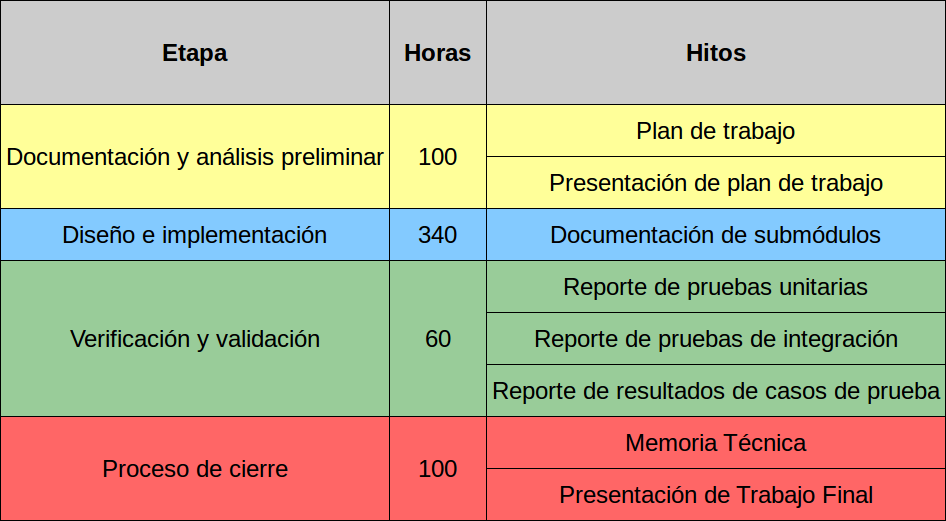
\includegraphics[width=\textwidth]{./Figures/planificacion.png}
%	\caption[Diagrama \textit{Etapas del proyecto}.]{Etapas principales del proyecto con el detalle de las horas planificadas y los hitos a alcanzar en cada una de ellas.}
%	\label{tab:planificacion}
%\end{table}

\begin{table}[ht]
	\centering
	\caption[Diagrama \textit{Etapas del proyecto}.]{Etapas principales del proyecto con el detalle de las horas planificadas y los hitos a alcanzar en cada una de ellas.}
	\begin{tabular}{lcl}
	\toprule
	\textbf{Etapa}   & \textbf{Horas} & \textbf{Hitos} \\ 
	\midrule
	\multirow{2}{*}{Documentación y análisis}  & \multirow{2}{*}{100}                     & Plan de trabajo                          \\
                                             &                                          & Presentación de plan de trabajo  \vspace{5px}        \\ \hline
	Diseño e implementación                    & 340                                      & Documentación de submódulos  \vspace{5px}            \\ \hline 
	\multirow{3}{*}{Verificación y validación} & \multirow{3}{*}{60}                      & Reporte de pruebas unitarias             \\
	                                           &                                          & Reporte de pruebas de integración        \\
	                                           &                                          & Reporte de casos de prueba       \vspace{5px}        \\ \hline
	\multirow{2}{*}{Proceso de cierre}         & \multirow{2}{*}{100}                     & Memoria Técnica                          \\
	                                           &                                          & Presentación de Trabajo Final            \\ 
	\bottomrule
	\end{tabular}
	\label{tab:planificacion}
\end{table}


Se realizó un desglose de tareas que puede verse esquemáticamente en el diagrama de \textit{Activity on Node} que se ilustra en la figura \ref{fig:AoN}. Se utiliza un mismo color para identificar las distintas tareas que componen una misma etapa del proyecto según la tabla \ref{tab:planificacion}. En color amarillo se detacan las tareas de la etapa de documentación y análisis; en celeste las tareas de diseño e implementación; en verde las tareas de verificación y validación y finalmente, en color rojo, las tareas que componen el proceso de cierre. En el diagrama, los tiempos de duración de las tareas están representados con la variable $t$ y expresados en horas. Asimismo, las tareas poseen un código numérico único que será usado para realizar la trazabilidad de los requerimientos.

\begin{figure}[ht]
	\centering
	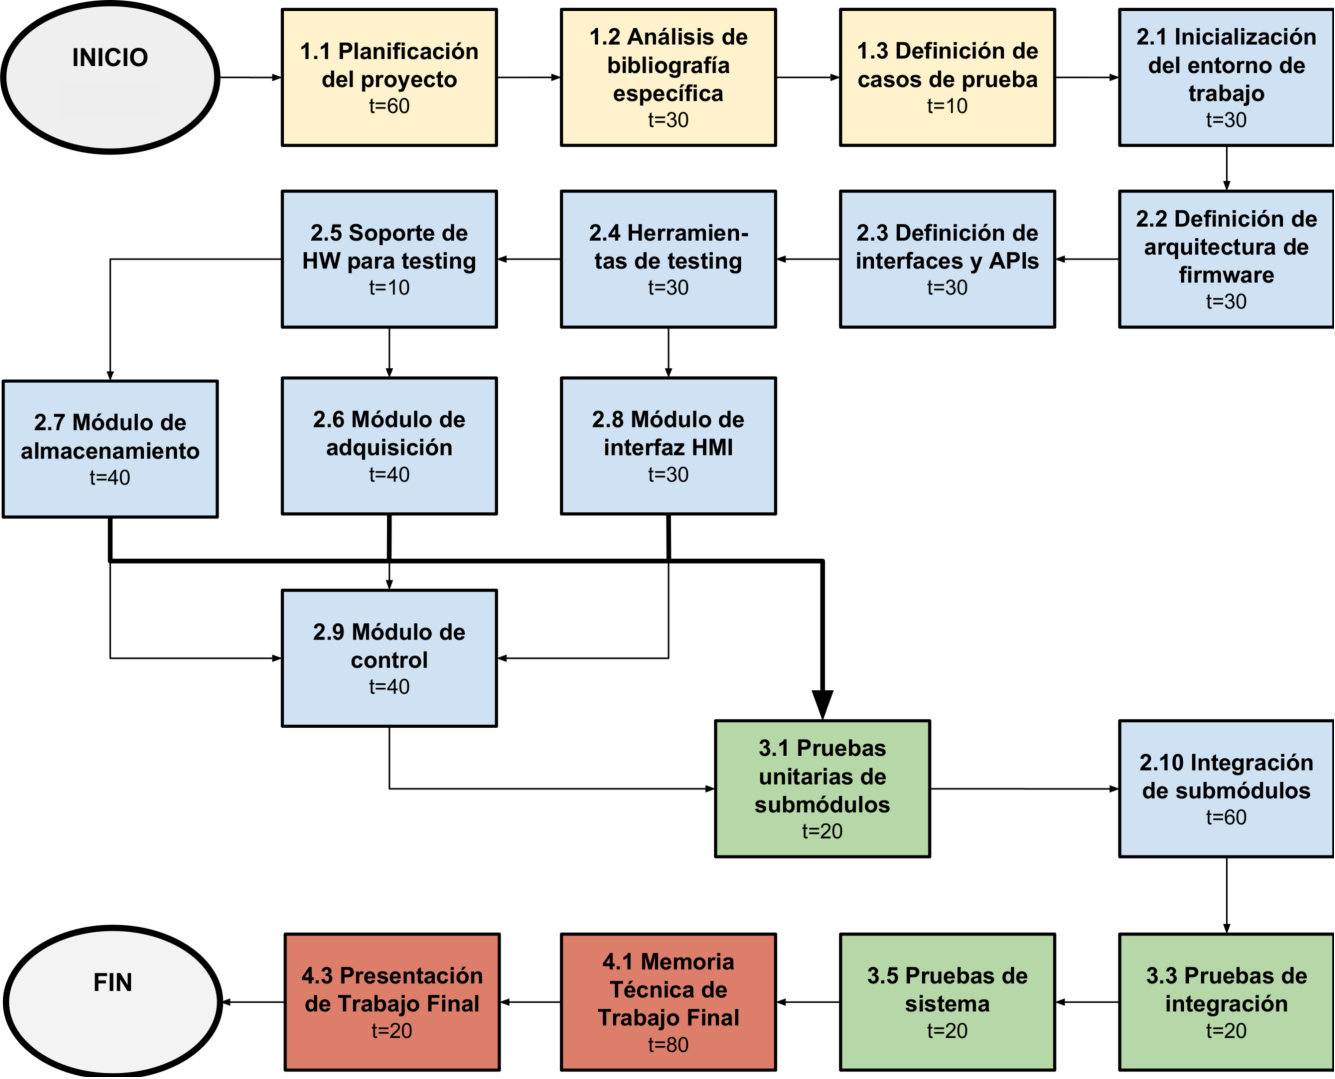
\includegraphics[width=\textwidth]{./Figures/AoN.pdf}
	\caption[Diagrama \textit{Activity on Node}.]{Diagrama \textit{Activity on Node}.  En colores pueden distinguirse las diferentes etapas del proyecto: en amarillo la etapa de documentación y análisis preliminar; en azul la etapa de diseño e implementación; en verde la etapa de verificación y validación y en rojo el proceso de cierre. El tiempo t está expresado en horas.}
	\label{fig:AoN}
\end{figure}

\clearpage
\section{Metodología}

En esta sección se describen los aspectos metodológicos relevantes que se aplicaron durante el desarrollo del trabajo.  

\subsection{Control de versiones}
\label{subsec:branching}

Se adoptó un modelo de desarrollo creado por Vincent Driessen llamado ``\textit{A successful Git branching model''} \citep{Driessen}.  El modelo está basado en la herramienta de control de versiones \textit{git} y consiste en un conjunto de procedimientos para ordenar y sistematizar el flujo de trabajo. Este modelo propone utilizar un repositorio considerado a los fines prácticos ``central'' (en git todos los repositorios son idénticos) llamado \textit{origin}.  Todos los desarrolladores trabajan contra este repositorio central con las operaciones típicas de \textit{push} y \textit{pop}.  

Adicionalmente, puede haber intercambios entre los repositorios de los distintos desarrolladores que formen un mismo equipo de trabajo. Estos intercambios pueden visualizarse en la figura \ref{fig:esquema-repos}, donde se esquematizan, por un lado, los posibles flujos de trabajo entre el repositorio \textit{origin} y los distintos desarrolladores, y por el otro, entre los repositorios propios de cada desarrollador. 

\begin{figure}[ht]
	\centering
	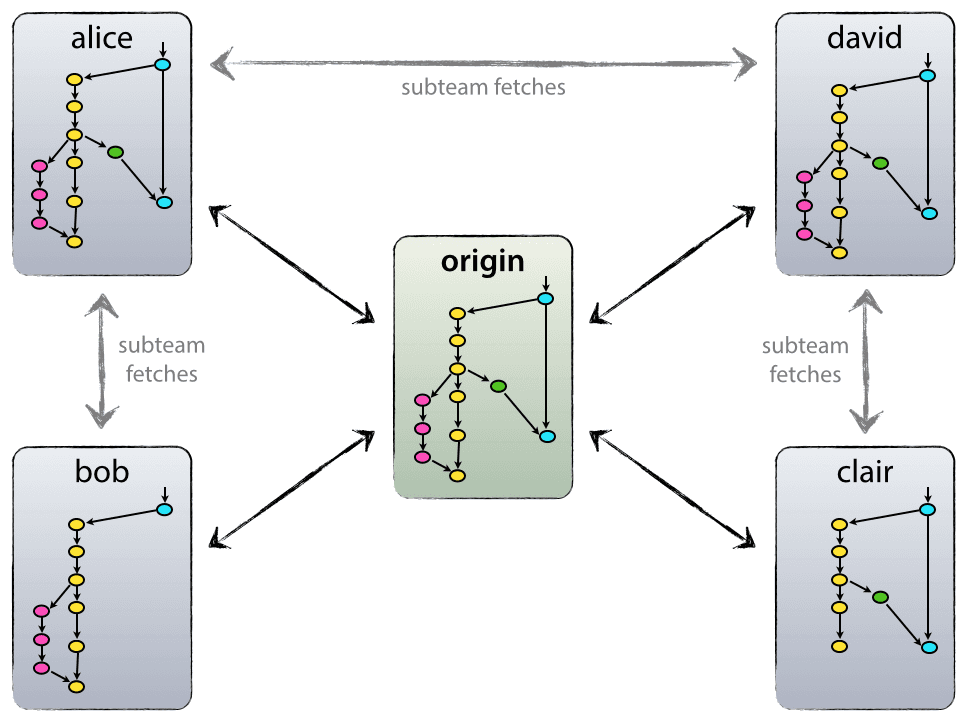
\includegraphics[width=.6\textwidth]{./Figures/centr-decentr@2x.png}
	\caption[Esquema del flujo de trabajo entre repositorios]{Esquema del flujo de trabajo entre repositorios\protect\footnotemark.}
	\label{fig:esquema-repos}
\end{figure}

\footnotetext{Imagen tomada de \url{https://nvie.com/img/centr-decentr@2x.png}.}

Para la elaboración de este trabajo, donde la codificación recayó principalmente sobre una sóla persona, no fueron habituales las operaciones contra un repositorio distinto de \textit{origin}, implementado en \textit{github}. Sin embargo, se considera la experiencia de apropiación de la metodología de trabajo muy valiosa para la formación profesional, ya que el autor de este trabajo no había tenido oportunidad de trabajar tan extensa y sistemáticamente con control de versiones previamente.

En cuanto a la estrategia de uso de ramas, siguiendo el modelo adoptado, se dispuso de dos ramas principales llamadas \textit{master} y \textit{develop}.  En \textit{origin/master} sólo se incluyen \textit{commits} con versiones estables con capacidad de ser puestas en producción, es decir sobre el prototipo de manera que éste pueda operar satisfactoriamente.  En \textit{origin/develop} se encuentran  los últimos cambios que integran las diferentes características ya logradas del código.  Cuando la rama \textit{develop} alcanza un punto de estabilidad y madurez suficiente se debe hacer un \textit{merge} con \textit{master}.% y generar un nuevo número de \textit{release}.

En términos generales, el esquema de ramas propuesto por el modelo de Vincent Driessen puede observar en la figura  \ref{fig:branching} donde se explicitan las posibles interacciones entre ramas.

\vfill

\begin{figure}[!htbp]
	\centering
	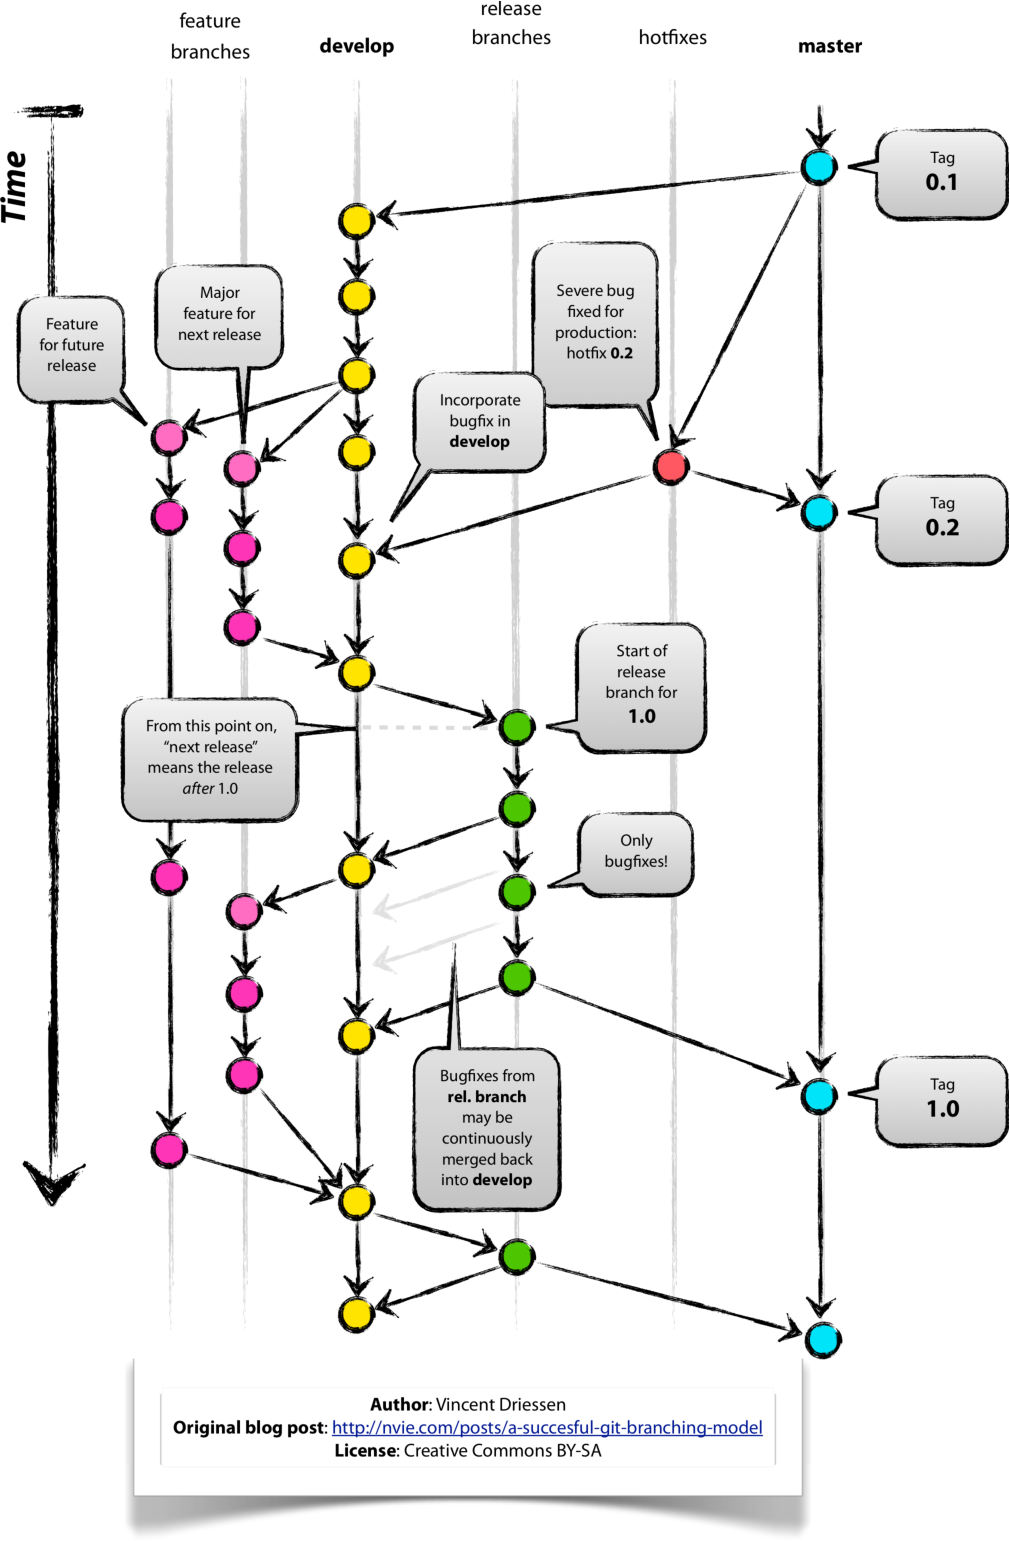
\includegraphics[width=.9\textwidth]{./Figures/Git-branching-model.pdf}
	\caption[Modelo de ramas utilizado en git]{Modelo de ramas utilizado en git\protect\footnotemark.}
	\label{fig:branching}
\end{figure}

\footnotetext{Imagen tomada de \url{https://nvie.com/files/Git-branching-model.pdf}.}

La mecánica de trabajo indica crear una nueva rama por cada característica a implementar.  Cuando la característica se logra, se debe hacer \textit{merge} con la rama \textit{develop} cuidando que no suceda un \textit{fastforward} y se pierdan los commits de la rama recién integrada.

Para este trabajo, se crearon ramas para desarrollar cada uno de los subsistemas mencionados en el diagrama en bloques de la figura \ref{fig:diagramaBloquesReducido} e incluidos en el alcance del trabajo, a saber:

\begin{itemize}
	\item \textit{sdcard} para el módulo de almacenamiento.
	\item \textit{onewire} para el módulo de adquisición.
	\item \textit{HMI} para el módulo de interfaz con el usuario.
	\item \textit{control} para el módulo de control.
	\item \textit{ceedling} para el entorno de testing.
\end{itemize}  



\subsection{Programación concurrente con Protothreads} 
\label{subsec:protothreads}

Los Protothreads son una abstracción creada por Adam Dunkel para implementar mecanismos de programación concurrente, conocidos como multi-tarea cooperativa, en sistemas embebidos con recursos limitados \citep{Protothreads}. 

Se distribuyen como una biblioteca que puede integrarse al proyecto y proveen la posibilidad de trabajar con hilos de ejecución sin \textit{stack} o co-rutinas, con mecanismos para bloquear la ejecución de una tarea sin que se produzca un cambio de contexto.  Esto permite un control de flujo secuencial sin máquinas de estado complejas o soporte multi-hilo completo en arquitecturas basadas en eventos \citep{dunkels06protothreads} \citep{dunkels05using}. 

En el presente trabajo, se hace uso de protothreads en la codificación del protocolo de comunicación 1-wire que se describe en la subsección \ref{subsec:1-wire}.